\chapter{基于模型融合的分心驾驶行为检测方法}


\section{引言}

随着时间的推移,视觉方向的研究逐渐从传统图像处理向卷积神经网络转变,硬件设备计算量的提升,使得其需要大计算量的算法得以验证。数据量的增多和算法性能的不断提升,致使交叉学科也在不断的迸发新的火花。分心驾驶行为检测的研究顺着时代的研究潮流,从生理信号的统计分析,转向使用成本低可靠的视觉分析。 

近些年分心驾驶行为检测算法在视觉方面的研究,也从传统机器学习的图像特征采集划分方式转向了深度学习更加可靠的端到端划分方式,性能方面得到了极大的提升。而且,深度学习也在前进发展的过程中,出现了交叉方向的融合研究方法(跨模态),例如跨模态学习、迁移学习和强化学习就是其中的代表之作。早期的分心驾驶行为由于数据集不公开,使得发表的方法难以浮现,普适性降低。2016年04月,著名的Kaggle在其竞赛网站公开了分心驾驶数据集,即StateFarm数据集,包含十种检测姿态(安全驾驶+九种分心驾驶行为),最终卷积神经网络(CNNs)被证明是最有效的方式\cite{46}。

自2012年以来,由于大量标记数据的可用性和计算能力,一批CNN网络,诸如AlexNet、ZFNet、VGGNet、GoogLeNet、ResNet等网络架构在视觉领域取得了非常好的成效。

2018年,Bhakti等人\cite{47}使用VGG在分心驾驶行为检测中取得了很好的成绩,并在其中加入了Dropout随机失活、L2权重正则化、BN批归一化。Bhakti针对VGG16参数量过高,全连接层消耗大量的计算资源,且不能应对不同输入图片等问题,使用1×1卷积进行替换,模型进行迁移学习,在大型分类数据集进行了预训练,在StateFarm数据集调优。

2019年,Chen等人\cite{49}。受Two-stream网络的启发,提出了利用一个空间流ConvNet提取空间特征和利用一个时间流ConvNet来捕获驾驶员的运动信息,应用特征融合方式整合不同模态的特征,进而使用ImageNet数据集进行预训练,迁移检测分类驾驶行为信息。

2020年09月,Gumaei等人\cite{50},通过使用边缘和云计算技术的深度学习方法来实时检测驾驶员的状态。该框架由三个模块构成,包括部署在车载环境边缘设备上的分心检测模块、部署在云环境中的训练模块和管理终端分析模块。算法主体由两个网络模型构建,一部分,自定义深度卷积神经网络(CDCNN);另一部分,基于视觉的微调VGG16网络模型。

分心驾驶作为视觉中的分类任务,属于经典的小类别任务(10分类)。深度卷积神经网络(CNNs)的对于特征的提取,可谓是得天独厚的优势,然而在视觉任务中,卷积网络还是没法对远距离关联的特征做出很好的响应。随着自然语言处理(NLP)中Transformer的盛行,视觉方面近些年也出现了基于Transformer网络模型,它能够很好的对远距离特征进行关联。因此本文是在此二者基础上,将卷积神经神经网络特征提取和视觉Transformer模型相融合,在数据集上进行评估。


\section{模型融合}

\subsection{ResNet网络}

深度学习的基础网络从AlexNet、VGG、GoogLeNet,模型结构随着任务强度的提升,网络卷积层数的数量也在增加。多层卷积结构能够进行更高级、更复杂的特征提取,简单的卷积层数增加会带来“梯度消失”和“梯度爆炸”问题。Kingming等人\cite{70}提出了深度残差网络结构(ResNet),成功解决了长时间训练网络难收敛问题和网络退化问题,使得网络层数更深的情况下,网络依然可以得到很好的性能与效率。

(1)	残差结构原理

残差结构是在输入与输出之间引入前向反馈。如图\ref{图3.1}所示,(a)全连接层在增加层数时将输入$x$映射为$h\left(x\right)=f\left(x\right)$;(b)残差结构输出是将$x$映射为$h\left(x\right)=f\left(x\right)+x$,即网络是在学习$f\left(x\right)=h\left(x\right)-x$,即$f\left(x\right)$被称之为残差项,当输入$x$与输出$h\left(x\right)$是维数相等时,输出$h\left(x\right)$与残差项$h\left(x\right)-x$等价。残差就是在原基础上,增加了一个跨层的连接,即x的恒等映射(Identity Mapping)。图\ref{图3.1}(b)是残差网络的基础结构,通过多层的连接结构组成瓶颈结构。对于输入x而言,可以更快的向前传播,或者反向传播(反向求导)。

\begin{figure}[!ht]
	\centering
	\subfloat[]{\includegraphics[height=5.33cm, width=4.86cm]{figures/图3.1.a.eps}%
		}
	\hfil
	\subfloat[]{\includegraphics[height=5.33cm, width=7.05cm]{figures/图3.1.b.eps}%
		}
	\caption{残差结构原理图}
	\label{图3.1}
\end{figure}


残差学习的原理如公式\ref{公式3-1}所示,

\begin{equation}\label{公式3-1}
	h\left(x\right)=f\left(x,\left\{W_i\right\}\right)+x
\end{equation}


$f\left(x,\left\{W_i\right\}\right)$表示拟合的残差项,且$x$与$f\left(x,\left\{W_i\right\}\right)$维数必须相等。若出现不等情形,则执行线性投影$W_s$来匹配维度或使用边缘填充技术来增加维度,如公式\ref{公式3-2}所示。

\begin{equation}\label{公式3-2}
	h\left(x\right)=f\left(x,\left\{W_i\right\}\right)+W_sx
\end{equation}

(2)	特征提取图

深度特征的类别区分,划分以其样本特征为主要手段,特征提取(Feature Extractor)的完备程度是决定判别器分类准确与否的先决条件,因此,好的分类算法同样也离不开判别器性能的影响。从人的认知角度出发,对于事物的区分,首先,是目标物体是否具有特殊的特征使人记忆犹新,能够根据特征很快确定出来;其次,针对其外观轮廓特征进行相匹配的甄别。

在深度学习的算法中,从设计理念出发,理想的网络模型能够提取到事物完整的特征,这些特征比人概略提取的事物特征数量更多。深度卷积是将整幅图进行相应的变换,经过不断的训练筛选出决定目标任务判别标准的主要特征,并不断的提升模型提取判别特征的能力,虽然这些特征最终融合为一种新的特征,人难以理解,但研究表明,确实判别器是能够判别。

图像作为多维数据,由于数据量太过庞大,直接送入判别器,很难做到精确的判别。深度学习模型提取特征,首先,是将其进行数据降维处理;其次,将提取到的特征进行筛选,在不断的训练中鉴别出具有决定作用的主要特征;最后,将融合在一起的新特征送入判别器进行判别。

\begin{figure}[!ht]
	\centering
	\subfloat[原图]{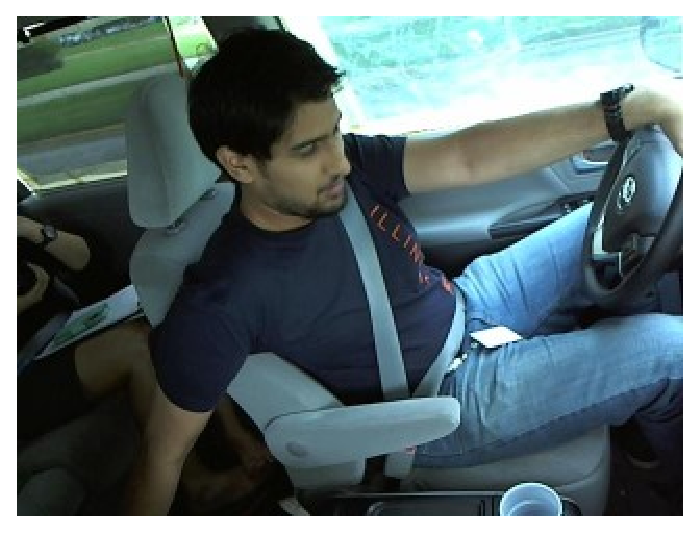
\includegraphics[height=5.29cm, width=5.06cm]{figures/图3.2a.eps}%
		}
	\hfil
	\subfloat[VGG特征图]{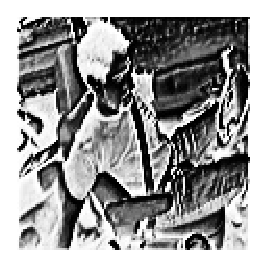
\includegraphics[height=5.29cm, width=5.06cm]{figures/图3.2b.eps}%
		}
	\hfil
	\subfloat[ResNet特征图]{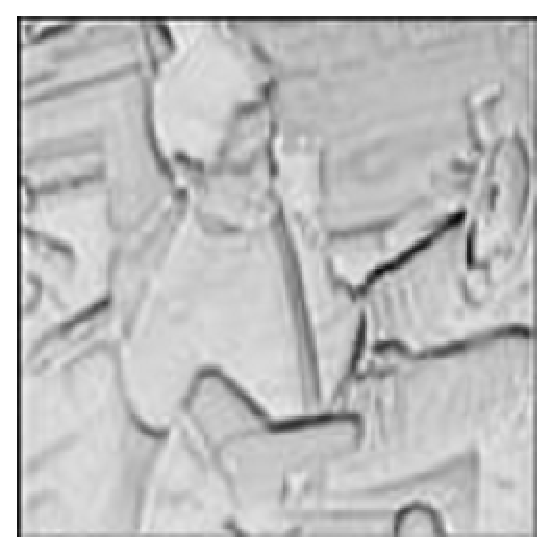
\includegraphics[height=5.29cm, width=5.06cm]{figures/图3.2c.eps}%
		}
	\caption{残差结构原理图}
	\label{图3.2}
\end{figure}


深度模型提取的图像的特征通过不断的运算融合,会使得提取到的特征更加抽象化,最终人类无法理解这些抽象化的特征,不可否认的是,目前的诸多研究表明,这些特征确实在判别器中能够被有效的鉴别,例如,人与动物对一件事物的区分,均会采用各自独有的特征理解方式,但不可否认,不同主体都可以鉴别事物的区分。由此可见,模型的判别能力现在已经超越了人为的判别能力。

\begin{figure}[!ht]
	\centering
	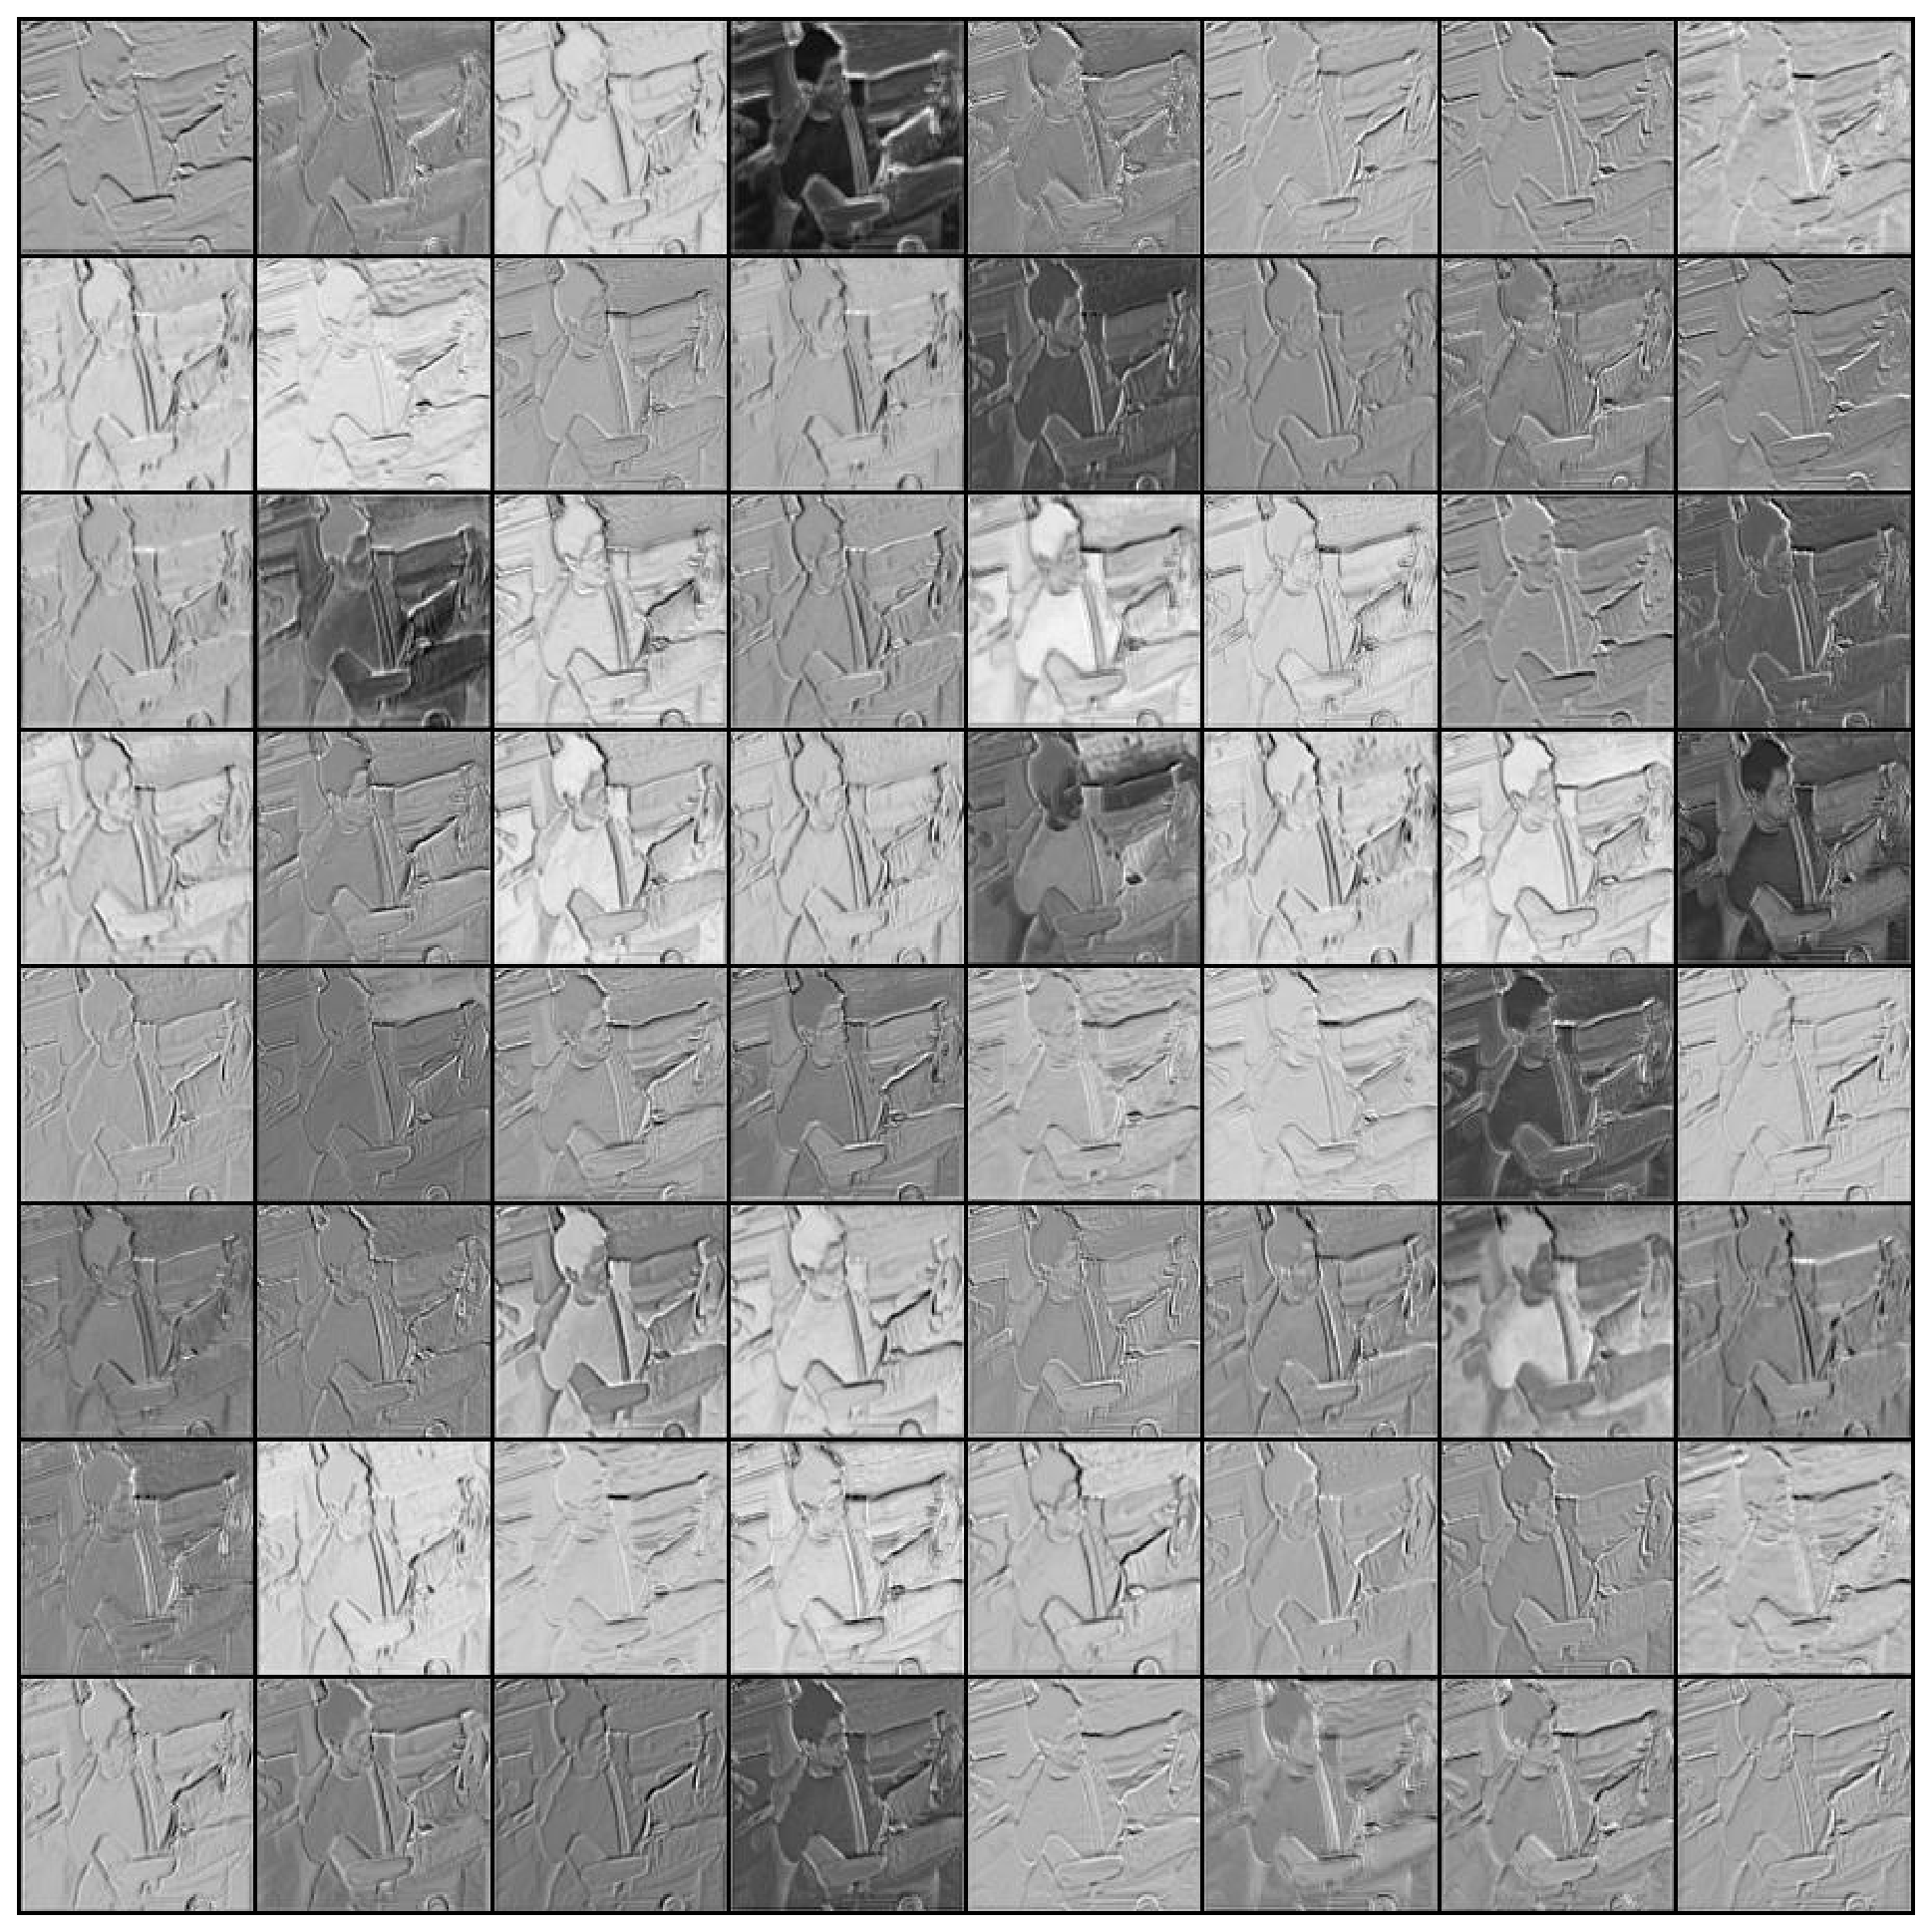
\includegraphics[height=7.66cm ,width=8.5cm]{figures/图3.3.eps}
	\caption{高斯滤波技术去噪示例}\label{图3.3}
\end{figure}

深度学习本质是将特征进行不断的卷积提取,得到更加复杂的信息。在此理论指导的前提下,模型对特征的提取能力是一个算法完成相应任务的前提,直接影响之后的任务完成度,如图\ref{图3.2}所示,使用的网络加载ImagNet数据集的权值文件,在State Farm进行调优,(a)是分心驾驶行为的模型鉴别输入原图,(b)将原图(a)输入经典的VGG16网络,第三层卷积处理特征效果图,(c)将原图(a)输入ResNet18网络,第三层卷积处理效果图。

从效果图可以明显的区分出,残差网络对于图像轮廓特征提取相对而言比较细腻,而VGG网络对于图像轮廓特征的提取明显是比较粗糙的,直接影响是残差网络的参数量较传统卷积深度堆叠的VGG网络而言更少,换而言之,即同样数量的参数,残差神经网络特征包含量远高于传统卷积深度堆叠的VGG网络,这会直接影响网络的训练时常和网络的参数复杂度。


残差网络从设计指出就决定了其在深层网络中的优势,即残差项在不断的训练学习过程中,可以更加有效的将有效特征信息向前映射,进而防止了有效特征信息在不断的训练过程中被模型抛弃丢失。如图\ref{图3.3}所示,ResNet卷积神经网络在ImageNet分类数据集上进行预训练,将图\ref{图3.2}(a)原图输入到ResNet网络中进行第三层卷积层的特征提取,可以明显的区分出,残差网络对于图像轮廓特征的提取,能够达到四分之三以上的有效性。轮廓特征在分心驾驶行为检测的分类任务中占据绝对主导的作用,且图\ref{图3.3}只是残差网络最浅层的ResNet18网络,随着残差网络的深度加深,特征提取效果会进一步的提升。

\subsection{Vision Transformer网络}

深度学习在自然语言处理(Natural Language Processing,NLP)方面一直是发展最好的,在实际工业应用中也是最完善的方向。其中Transformer是最早应用在自然语言处理邻域\cite{51},Transformer不同于以往的CNN卷积神经网络和循环神经网络RNN,整个网络完全是由自注意力机制(self-Attenion)和前馈神经网络(Feed Forward Neural Network)构成,用于提取内在特征。由于Transformer网络编码器和解码器(Encoder-Decoder)在一维线性特征上的优势问题,NLP在机器翻译中取得了最佳无偏估计(Best Linear Unbiased Estimator,BLUE)值的新高度。

视觉任务相比于文本任务,视觉涉及到更大的尺寸、图像噪声和冗余信息,因此Transformer很难直接去适用视觉任务。最近,随着Transformer在计算机视觉方面也发展迅猛,例如目标检测的DETR\cite{52},语义分割的SETR\cite{54}和图像识别的VIT\cite{53}和DeiT\cite{55}。

(1)	Vision Transformer基础原理

基于视觉的Transformer模型主要是以处理二维数据图像为主,与卷积神经网络(CNNs)相比,可以能有效地发掘特征之间的远距离依赖关系。在NLP领域Transformer的指导下,将二位图像进行构建图像序列,即将图像进行切割分块,这种图像序列隐含了图像局部特征之间远距离的依赖关系。

图像分类作为计算机视觉任务的核心之一,经常用于衡量图像任务研究进展的基础标准,检测和分割任务都是在此基础上进行改进。ImageNet分类数据集检测性能的提升代表着神经网络结构的研发进展。

标准的Transformer输入接受的是一维融合多组信息的序列,对于二维图像而言,是将一副图像进行切割成块,将其位置信息、标签信息和切割成的块图像融合成一个序列,再输入进图像中,如下公式(\ref{公式3-3})所示:


\begin{equation}\label{公式3-3}
	\mathbf{x} \in R^{H \times W \times C} \Leftrightarrow \mathbf{x}_{p} \in R^{H \times\left(P^{2} \cdot C\right)}
\end{equation}

其中,$\left(H,W\right)$图像原尺寸,C是通道数,$\left(P,P\right)$是扁平化的每个图像块尺寸。
图像切割之后个序列块与原图像尺寸相互关系如公式(\ref{公式3-4})所示:

\begin{equation}\label{公式3-4}
	N=\frac{HW}{P^2}
\end{equation}

其中,$N$是将$H\times W\times C$尺寸的图像转换为扁平化块尺寸为$\left(P,P\right)$图像块的个数,同时$N$也是Transformer有效输入长度。

\begin{figure}[!ht]
	\centering
	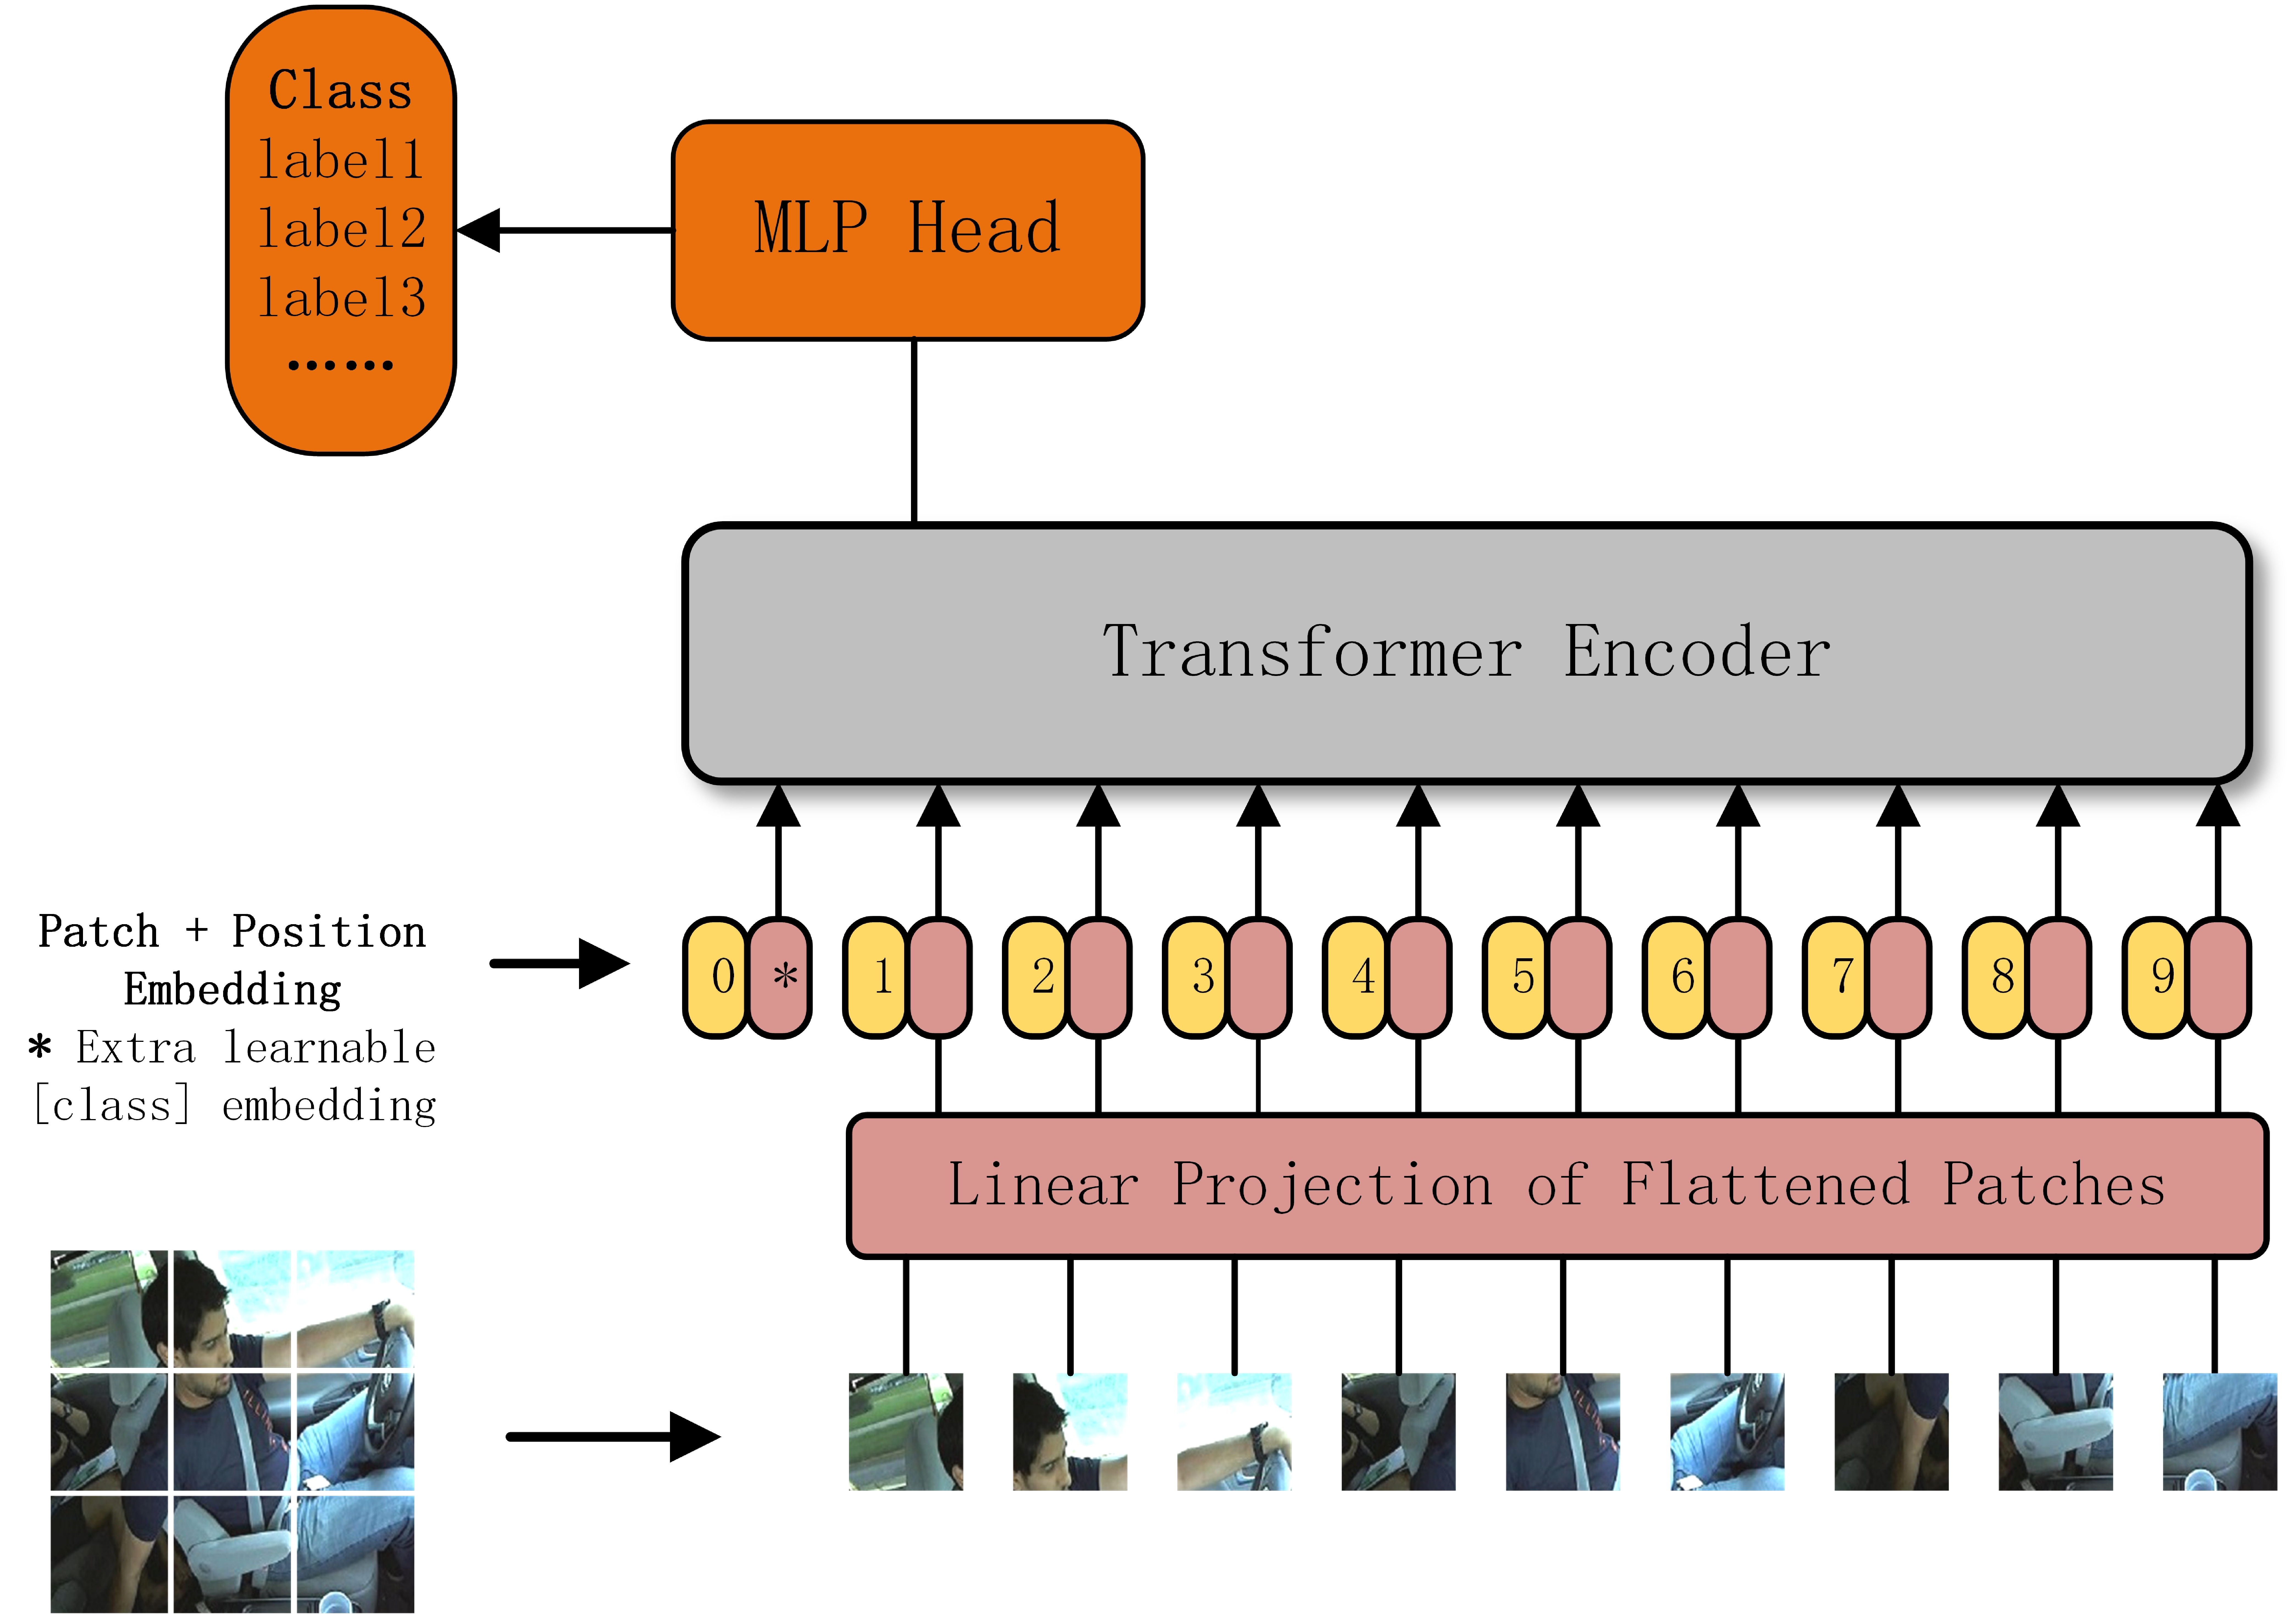
\includegraphics[height=9.34cm ,width=13.27cm]{figures/图3.4.eps}
	\caption{基于视觉的Transformer模型原理图}\label{图3.4}
\end{figure}


图像在转换为序列块时,受块的尺寸$\left(P,P\right)$大小变换的影响,每个转换后的序列$\left(P^2C\right)$维度的向量长度也会变换,为避免模型结构扁平化块尺寸$\left(P,P\right)$的影响,如公式(\ref{公式3-5})所示,对扁平化序列向量做线性映射(Linear Projection of Flattened Patches),即将扁平化序列块映射到固定的D维向量。

\begin{equation}\label{公式3-5}
\mathbf{z}_0=\left[\mathbf{x}_{\mathrm{class}},\mathbf{x}_p^1\mathbf{E},\mathbf{x}_p^2\mathbf{E},\cdots,\mathbf{x}_p^N\mathbf{E}\right]+\mathbf{E}_{pos},\mathbf{E}\in R^{\left(P^2.C\right)\times D},\mathbf{E}_{\mathrm{pos}}\in R^{\left(N+1\right)\times D}
\end{equation}

Transformer编码器由公式(\ref{公式3-6})多头注意力机制和公式(\ref{公式3-7})多层感知机的交替构成。如图\ref{图3.5}所示,在每一块之前使用公式(\ref{公式3-8})层标准化,在每一块之后使用残差连接。


\begin{equation}\label{公式3-6}
	\mathbf{z}_l^\prime=MSA\left(LN\left(\mathbf{z}_{l-1}\right)\right)+\mathbf{z}_{l-1},\ \ l=1\ldots L
\end{equation}

\begin{equation}\label{公式3-7}
	\mathbf{z}_l=MLP\left(LN\left(\mathbf{z}_l^\prime\right)\right)+\mathbf{z}_l^\prime,\ \ l=1\ldots L
\end{equation}


\begin{equation}\label{公式3-8}
	\mathbf{y}=LN\left(\mathbf{z}_L^0\right)
\end{equation}

(2)	Vision Transformer网络模型结构

基于视觉的Transformer网络模型结构(Vision Transformer,VIT)是基于自然语言处理NLP的Transformer模型原理更改过来,由于注意力机制在视觉任务中的有利优势,各种ResNet-like(添加了注意力机制)模型在测试中的性能优异表现,使得视觉开始转向注意力机制的源头自然语言处理NLP的Transformer模型,Transformer模型天生自带自注意力机制,和其远距离特征的联系,使得视觉的Transformer网络模型结构VIT模型提出之后,性能上逐渐追平了SOTA模型。


\begin{figure}[!ht]
	\centering
	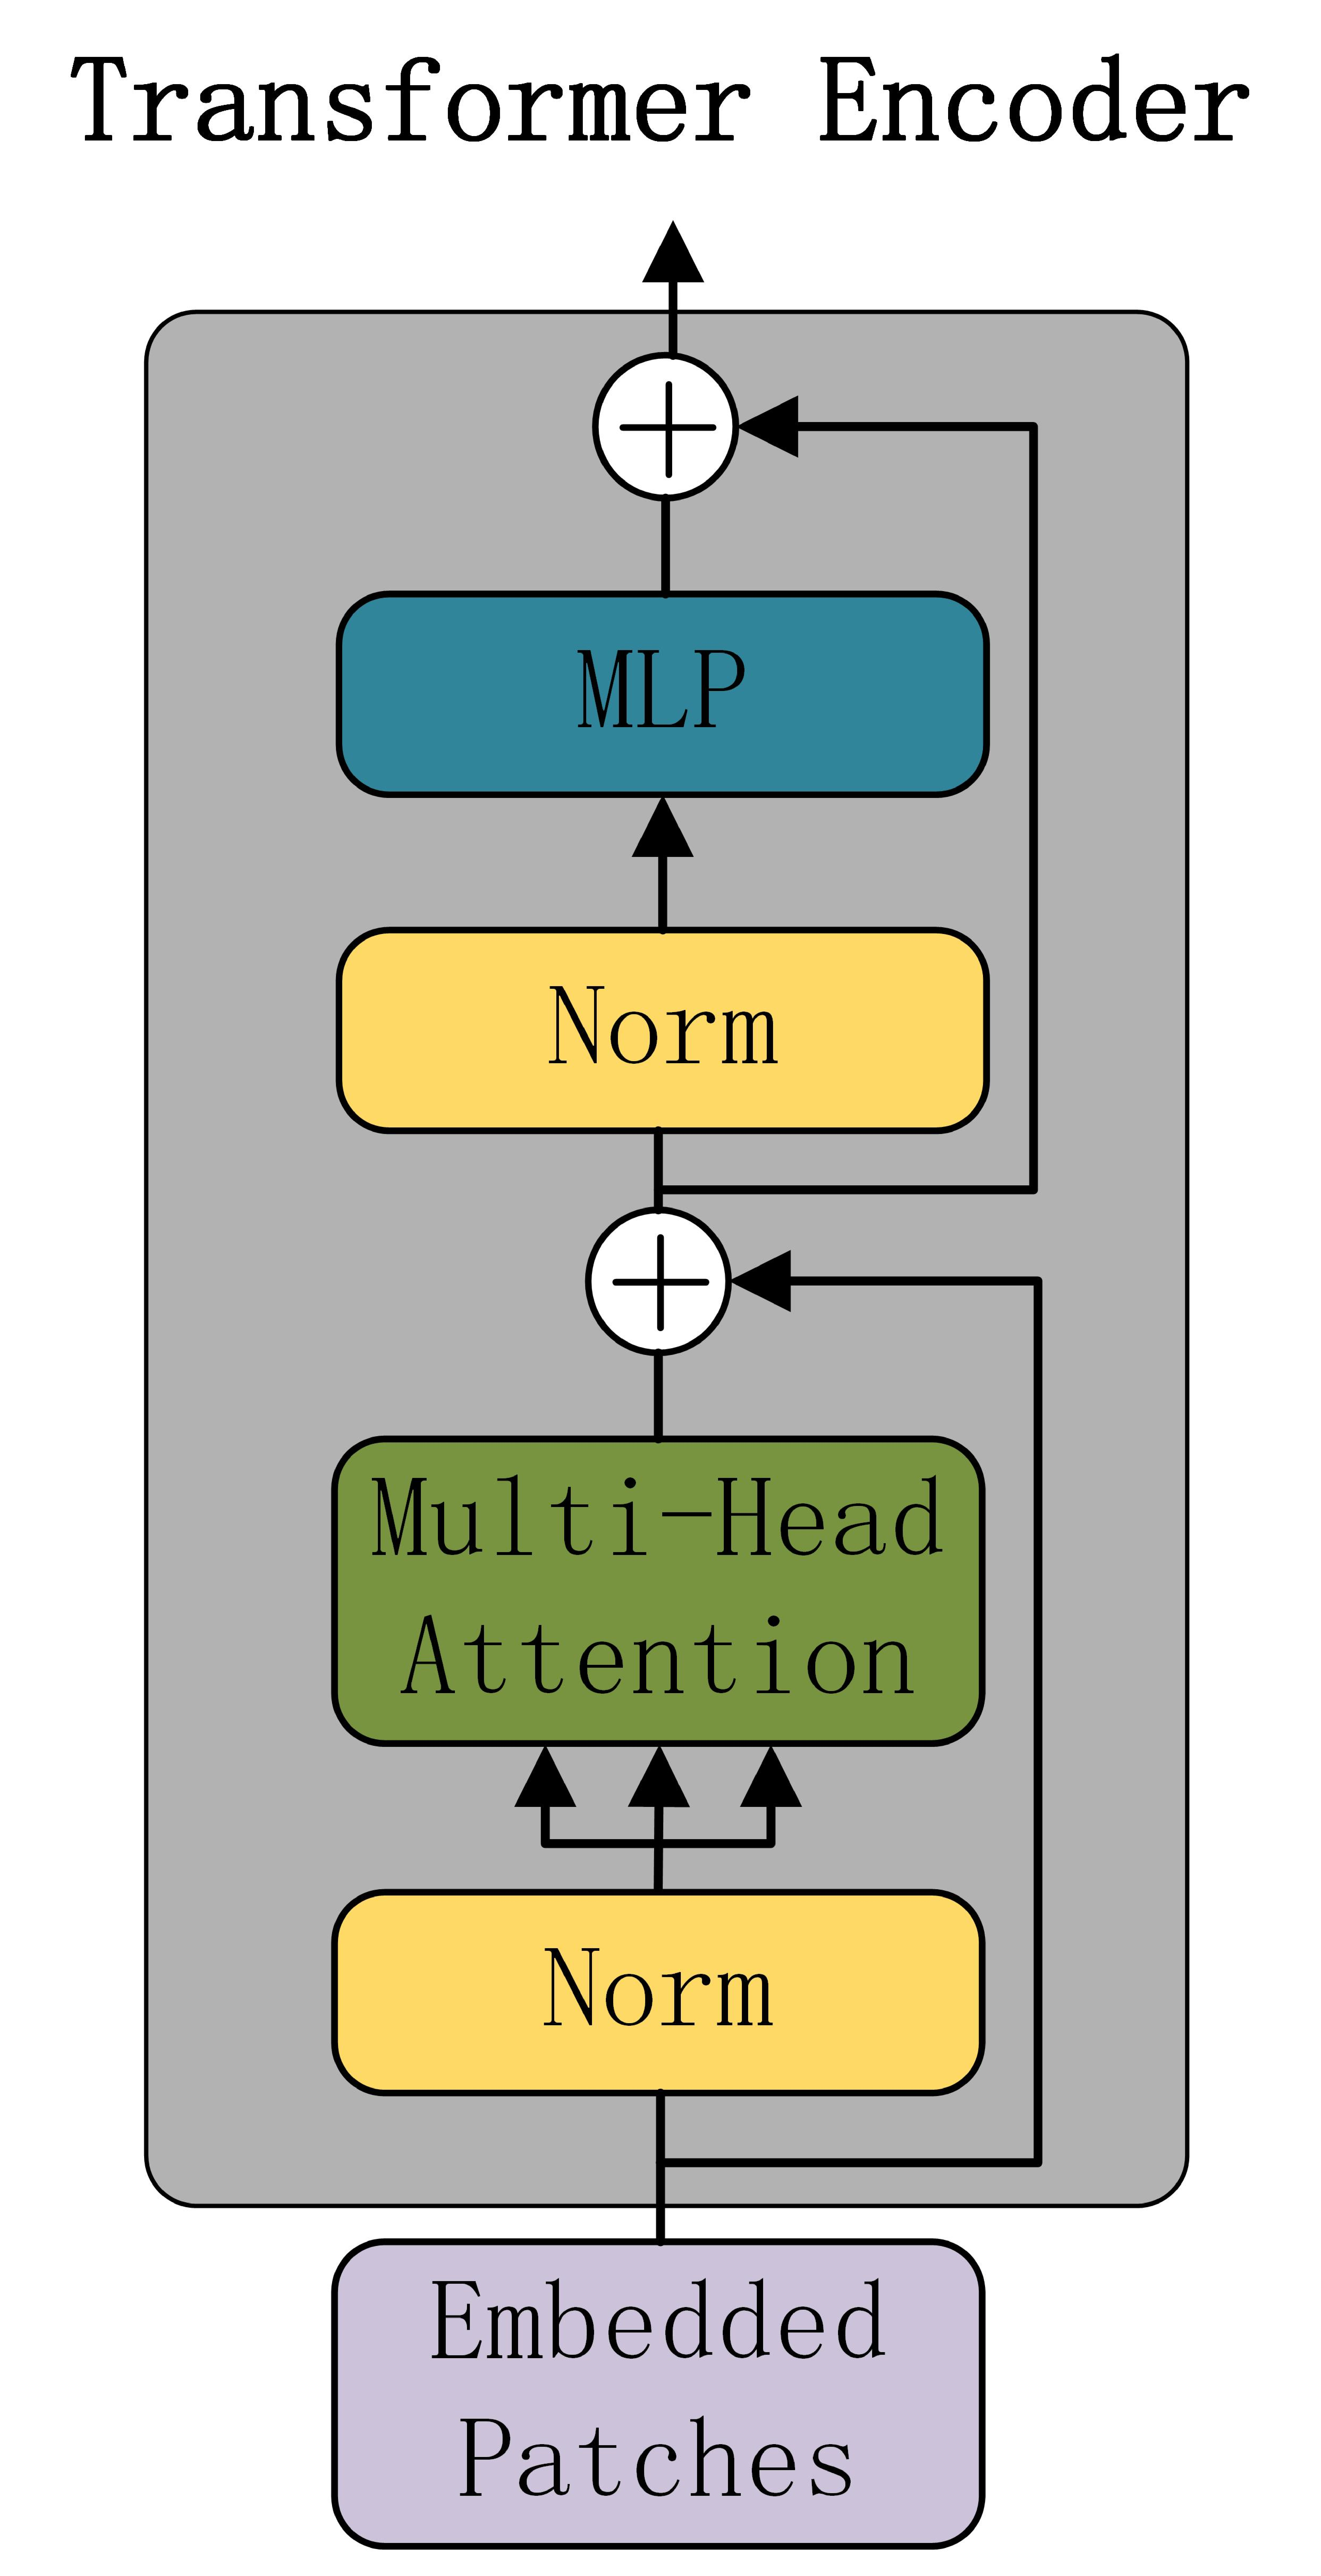
\includegraphics[height=9.22cm ,width=4.87cm]{figures/图3.5.eps}
	\caption{Transformer编码器结构}\label{图3.5}
\end{figure}

VIT的网络结构如图\ref{图3.4}所示,首先将输入图像分割成固定大小的图像块,为了使得VIT模型能够接受任意尺寸的输入图像,在序列向量输入Transformer编码器之前,对扁平化的图像块进行$D$维线性映射。其次,模型再将每个分割后的块进行线性嵌入位置信息,组成序列为$D$维的向量,为了使得训练之后的模型可以进行相应的分类任务,因此在向量序列中添加一个额外的分类学习的标签信息(公式(\ref{公式3-5})中向量维数$N+1$,其中$N$是分割后的图像块数目,1是额外添加的分类学习标签信息),即图中位置为0嵌入信息“*”表示额外的分类标签信息(公式(\ref{公式3-5}),$\symbfit{z}_0^0=\symbfit{x}_{\mathrm{class}}$),如公式(\ref{公式3-8})所示,其在Transformer编码器($\symbfit{z}_L^0$)输出的$\mathbf{y}$表示整张图像的输出结果。最后,Transformer编码器进行编码,结果经过MLP运算得到最终类别输出。

\subsection{RViT网络}

在过去几年的研究中,分心驾驶行为检测的检测仍旧以卷积神经网络CNN为主,卷积神经网络对于特征的提取具有得天独厚的优势,是其他网络模型所不能媲美的。Transformer在分心驾驶行为检测方面还是未被关注。然而,基于模型特征的分心驾驶分类任务,已经不满足于局部特征的单一鉴别,即驾驶姿态多部位特征之间的关联是分类任务性能提升的又一个方向。

Transformer具有高效的计算性能和可扩展性能,现如今的视觉领域(CV)还是以ResNet-like结构为主,虽然ViT和DeiT等模型的出现使得性能方面逐渐能够与ResNet等网络相媲美,甚至某些方面能够超过ResNet网络,但距离追赶更高性能的SOTA(ResNet-like)网络还是有差距。

本文是在基于视觉的Transformer网络(ViT)的基础上,分析ViT网络存在的图像特征提取不完备问题和输出线性层参数量过大存在的过拟合问题出发,根据ResNet模型提取特征性能优异的表现及ViT网络对于长远距离的局部特征关联性出发,提出了基于ResNet网络和Vision Transformer网络(Residual Vision Transformer,RViT)融合的网络模型。

\begin{figure}[!ht]
	\centering
	\includegraphics[height=7.35cm ,width=15.5cm]{figures/图3.6.eps}
	\caption{ResNet与Transformer模型融合的网络示意图}\label{图3.6}
\end{figure}

由于基于视觉的Transformer(ViT)网络模型在预训练过程中消耗的资源和时间,本文将在基于视觉的Transformer(ViT)的另一个变种DeiT网络的基础上,尽可能的遵守原始DeiT的设计规则。如\ref{图3.6}所示,取缔了DeiT的蒸馏令牌(Distillation Token),保留了Transformer模型的自注意力机制、多头自注意力机制和多层感知机,可以直观的使用DeiT的预训练权重,对模型进行修改进行迁移学习,可达到同样的效果。

RViT首先是使用ResNet对模型进行粗略特征的提取,其次是遵循视觉Transformer(ViT)的理念,将卷积得到的特征图像序列化(Feature Serialization)处理,为了减少网络模型参数过量而引起的过拟合问题和模型准确率下降问题,进行一次序列块局部平均池化(Local Average Pooling)运算,即在保持序列化特征图像块抽象特征足够的前提下,对切割后的特征图像块进行局部特征值平均池化。减少特征参数,保留序列块整体轮廓特征,加快了模型的收敛速度,提升了模型分类准确率。


不同于自然语言处理NLP的Transformer模型中$cos-sin$的位置编码方式。ViT采用的时随机初始化生成的位置参数,在模型训练中不断的学习参数。输入Transfomer编码器的参数由ResNet卷积输出的分割块参数、特征位置参数和数据标签类别参数共同组成。如公式(\ref{公式3-9})、公式(\ref{公式3-10})所示:

\begin{equation}\label{公式3-9}
	x_{pt}=Conv\left(x\right)+x_{pos}
\end{equation}

\begin{equation}\label{公式3-10}
	x_{class}=W^c                         
\end{equation}

其中,$x$为ResNet卷积特征输出分割块序列,$x_{pos}$为特征分割块的位置参数,$x_{pt}$为组成的特征序列块,$x_{class}$为特征序列块的类别特征,$W^c$为可训练的序列化向量。


\section{仿真实验}

\subsection{实验设置}

本章实验在Windows平台,借用Python的跨平台特性,运行在一台Dell服务器上,详细配置如下:

CPU:Intel Xeon Silver 4110 @ 2.20GHz

内存:64 GB

显卡:NVIDIA GeForce RTX 3090

系统:Windows10专业工作站版本

框架:PyTorch1.7

(1)	实验数据集

本章为评估RViT网络分类性能,主要在以下几个数据集上进行了训练和测试,驾驶行为检测方面,如表\ref{表3.1}所示,选用了Kaggle公开的StateFarm分心驾驶行为检测数据集,与StateFarm数据集分布类似的AUCD2分心驾驶行为检测数据集。为验证RViT数据集本身的性能,选用了同类型任务的分类数据集CIFAR-10、ImageNet、CIFAR-100分类数据集做性能的辅助评估测试。

StateFarm数据集包含有10个类别共102150张图像,分别为用于训练的22424张图像和用于测试的79726张,训练分心样本包括安全驾驶2489张、右手打字2267张、右手接电话2317张、左手打字2346张、左手接电话2326张、调收音机2312张、喝饮料2325张、拿后面东西2002张、整理头发和化妆1911张和与乘客交流2129张,测试集没有标签文件,需要在Kaggle平台评估打分。


% Please add the following required packages to your document preamble:
% \usepackage{multirow}
\begin{table}[!ht]
	\caption{StateFarm和AUCD2分心驾驶行为数据集的分布}
	\label{表3.1}
	\renewcommand{\arraystretch}{1.5}
	\centering
	\begin{tabular}{p{2.5cm}<{\centering}p{3.5cm}<{\centering}p{2.5cm}<{\centering}p{2.5cm}<{\centering}}
		%\hline
		\bottomrule
		\multicolumn{1}{c}{\multirow{2}{*}{类别编号}} &  \multicolumn{1}{c}{\multirow{2}{*}{类别名称}} & \multicolumn{2}{c}{图片数量}                                  \\ \cline{3-4} 
		\multicolumn{1}{c}{}                      & \multicolumn{1}{c}{}                      & \multicolumn{1}{c}{StateFarm} & \multicolumn{1}{c}{AUCD2} \\ \hline
		CO                                        & 安全驾驶                                      & 2489                          & 3686                      \\
		C1                                        & 右手打字                                      & 2267                          & 1974                      \\
		C2                                        & 右手接电话                                     & 2317                          & 1223                      \\
		C3                                        & 左手打字                                      & 2346                          & 1301                      \\
		C4                                        & 左手接电话                                     & 2326                          & 1361                      \\
		C5                                        & 调收音机                                      & 2312                          & 1220                      \\
		C6                                        & 喝饮料                                       & 2325                          & 1612                      \\
		C7                                        & 拿后面东西                                     & 2002                          & 1159                      \\
		C8                                        & 整理头发和化妆                                   & 1911                          & 1202                      \\
		C9                                        & 乘客交流                                      & 2129                          & 2570                      \\
		\bottomrule
	\end{tabular}
\end{table}

AUCD2数据集包含7名不同国家的31个驾驶人员的数据,AUCD2共有10个类别17303张图像,包括安全驾驶3686张、右手打字1974张、右手接电话1223张、左手打字1301张、左手接电话1361张、调收音机1220张、喝饮料1612张、拿后面东西1159张、整理头发和化妆1202张和与乘客交流2570张,拥有训练集标签和测试机标签文件。

CIFAR-10数据集是一个接近普适分类3通道的RGB彩色数据集,其拥有10类共60000张图像,用于训练和测试图像分别是50000张和10000张。

ImageNet数据集是一个大型综合性的视觉数据集,使用ImagNet2012数据集包含1000多个分类,比如:“气球”、“轮胎”和“狗”等,数据集总共含有140多万张图像,每个分类不少于500张。

(2)	图像预处理

本章所使用的模型RViT,由于扁平化线性映射层(Linear Projection of Flattened Patches)的存在,对于模型输入图像尺寸不再做处理。在训练阶段,为了增强数据,使用10-crop方式,对数据进行范围为($-{10}^\circ,{10}^\circ$)的随机饭庄,且以50\%的概率随机水平翻转。

训练数据集统一将图像转换成224×224×3的尺寸,采用随机梯度下降法对模型进行端对端训练,每批128个训练样本,动量矩参数为0.9,采用的Heinitialization方法初始化卷积网络系数,L2正则系数为$3×10^{-4}$,迭代次数为200,初始学习率为0.01,使用CosineAnnealingLR进行学习率更新。本章的RViT与ViT使用迁移学习,所在ImageNet大型数据集上进行训练,在各数据集上进行微调。

训练数据集统一将图像转换成224×224×3的尺寸,每批32个测试样本,统计每次训练的数据变化作准确率与稳定度度量。

\subsection{性能评价标准}


本文采用文献\cite{66}中的平均准确率和稳定度两个标准。对每种方法测试$N$($N=10$)次,以$N$次结果的平均值作为最终准确率,定义为:

\begin{equation}\label{公式3-11}
	Acc=\frac{\sum_{i=1}^{N}{Acc}_i}{N}
\end{equation}

${Acc}_i$是第i次实验的识别率。由于网络参数随机初始化和训练样本随机分批的原因,相同设置下每一次的识别结果有一定的误差,所以,采用多次实验的平均值更加公平可靠。

稳定度是N次实验结果的均方差,定义为:

\begin{equation}\label{公式3-12}
	S=\sqrt{\frac{\sum_{i=1}^{N}\left(Acc_i-Acc\right)^2}{N}}
\end{equation}

稳定度S体现了相同设置下实验结果的变化程度,S越小,表明模型性能越稳定。

\subsection{实验结果及分析}

本章使用经典的卷积神经网络(CNN)有VGG、AlexNe、InceptionV3、Modified VGG(M-VGG)、ResNet,基于视觉的Transformer网络(ViT)和基于ResNet和ViT融合的RViT网络模型进行对比。

\begin{table}[!ht]
	\caption{RViT与ViT的参数详情}
	\label{表3.2}
	\renewcommand{\arraystretch}{1.5}
	\centering
	\begin{tabular}{cccccc}
		\bottomrule
		模型       & 序列块数量 & 序列块大小   & 隐藏层特征 & 多层感知机特征 & 多头注意力机制 \\ \hline
		RViT/ViT & 8    & (16,16) & 768   & 1024    & 8      \\ 
		\bottomrule
	\end{tabular}
\end{table}

% Please add the following required packages to your document preamble:
% \usepackage{multirow}
\begin{table}[!ht]
	\caption{各分类算法在数据集中准确率(Acc)的性能比较}
	\label{表3.3}
	\renewcommand{\arraystretch}{1.5}
	\centering
	\begin{tabular}{p{2.5cm}<{\centering}p{2.5cm}<{\centering}p{2.5cm}<{\centering}p{2.5cm}<{\centering}p{2.5cm}<{\centering}}
		\bottomrule
		\multirow{2}{*}{方法} & \multicolumn{4}{c}{准确率(Acc/\%)}                                                                               \\ \cline{2-5} 
		& StateFarm                 & AUCD2                     & CIFAR-10                  & ImagNet                   \\ \midrule
		\multicolumn{5}{c}{卷积神经网络(Convnets)}                                                                                                \\ \midrule
		VGG16               & 71.51                     & 94.44                     & 92.19                     & 65.67                     \\
		AlexNet             & 70.72                     & 93.65                     & 87.46                     & 61.32                     \\
		InceptionV3         & 73.85                     & 95.17                     & 92.42                     & 75.80                     \\
		M-VGG               & 72.34                     & 95.54                     & —                         & —                         \\
		ResNet18            & 72.49                     & 96.52                     & 91.02                     & 69.82                     \\
		ResNet50            & 75.92                     & 97.64                     & 92.62                     & 76.23                     \\ \midrule
		\multicolumn{5}{c}{Vision Transformer网络}                                                                                            \\ \midrule
		ViT                 & \multicolumn{1}{l}{81.43} & \multicolumn{1}{l}{98.75} & \multicolumn{1}{l}{97.13} & \multicolumn{1}{l}{77.91} \\
		RViT                & \multicolumn{1}{l}{82.35} & \multicolumn{1}{l}{99.36} & \multicolumn{1}{l}{98.37} & \multicolumn{1}{l}{79.47} \\ \bottomrule
	\end{tabular}
\end{table}

(1)	模型分类准确率

实验所使用的ViT和RViT是基于BERT\cite{56}的配置,详细信息如表\ref{表3.2}所示,序列块的数量为8,序列块大小为(16,16),隐藏层特征768,多层感知机的特征为1024(是隐藏层特征的2倍),多头注意力机制(MSA)的Heads参数为8。注意,VisionTransformer模型的序列块大小与块的数量成反比,块较小的模型计算成本高。

实验网络模型是按照论文原文,由PyTorch文档提供,未加任何修改。从表\ref{表3.3}可以明确的观察到,在最重要的准确率(Acc/\%)指标中,基于视觉的Transformer网络较卷积神经网络(CNN)而言,整体都表现出相当不错的性能。

StateFarm分心驾驶行为数据集方面,由于测试集图像数量远多于训练集,因此各网络模型算法的性能表现欠佳。其中,卷积神经网络中ResNet50网络模型准确率达到75.92,表现最为良好,Vision Transformer网络中RViT网络模型的准确率达到82.35,较同类型的ViT网络提升0.92,但却比卷积神经网络最好的模型ResNet50高6.43。

AUCD2分心驾驶行为数据集方面,卷积神经网络中ResNet50网络模型表现最为良好,准确率达到97.64,Vision Transformer网络中RViT网络模型的准确率达到99.36,较同类型的ViT网络提升0.09,但却比卷积神经网络最好的模型ResNet50高2.09。

CIFAR-10分类数据集方面,卷积神经网络中ResNet50网络模型准确率达到92.62,Vision Transformer网络中RViT网络模型的准确率达到99.37,较同类型的ViT网络提升0.24,但却比卷积神经网络最好的模型ResNet50高6.75。

ImageNet分类数据集方面,卷积神经网络中ResNet50网络模型准确率最高,达到76.23,Vision Transformer网络中RViT网络模型的准确率达到79.47,较同类型的ViT网络提升1.56,但却比卷积神经网络最好的模型ResNet50高3.24。

\begin{figure}[!ht]
	\centering
	\includegraphics[height=8.35cm ,width=12.58cm]{figures/图3.7.eps}
	\caption{在AUCD2数据集上,残差网络与Vision Transformer训练准确率对比}\label{图3.7}
\end{figure}

综上所示,本文提出的RViT网络特性上,仍旧是以Transformer网络为主体,Vision Transformer网络模型能有如此优异的准确率性能表现,得益于模型对远距离特征之间的相互联系性,这也是卷积神经网络在分类任务中一直所欠缺的。而且,RViT网络在ViT网络的基础性能由稍微的提升,与本文的设计思路相吻合,得益于ResNet残差结构对特征的提取,Transformer将远距离特征之间的关系结合起来,最终使得模型的性能得到提升。

(2)各模型准确率变化情况

卷积神经网络和Transform网路在训练过程中,如\ref{图3.7}所示,在整体的训练迭代中,选择迭代次数40次以后的训练权重进行测试。残差网络网络深度对于准确率的影响较为明显,网络深度与时间成正比。Vision Transform网络整体准确率较残差网络较高。RViT网络对着迭代次数的增多,模型的震荡较ViT网络更缓和。


(3)	模型稳定度

各网络模型在稳定度(S)方面,即网络模型的稳定度越小,模型准确性能波动越小,越稳定。从表\ref{表3.4}中可以明确的观察到,在StateFarm分心驾驶行为数据集上,卷积神经网络的稳定性整体稍逊于Vision Transformer网络,然而,单个模型稳定度上,ResNet50的稳定效果最佳,达到了0.408。在AUCD2分心驾驶行为数据集上,卷积神经网络的稳定性整体强于Vision Transformer网络,其中Modifed VGG的稳定效果最好,达到了0.174。并且,分心驾驶行为数据集StateFarm的稳定度整体较AUCD2数据集高,波动程度的影响与数据集的训练图像和测试图像的比例分布有直接的联系。


% Please add the following required packages to your document preamble:
% \usepackage{multirow}
\begin{table}[!ht]
	\caption{各分类算法在分心驾驶行为数据集中稳定度(S)的性能比较}
	\label{表3.4}
	\renewcommand{\arraystretch}{1.5}
	\centering
	\begin{tabular}{p{3.75cm}<{\centering}p{3.75cm}<{\centering}p{3.75cm}<{\centering}}
		\bottomrule
		\multicolumn{1}{c}{\multirow{2}{*}{方法}} & \multicolumn{2}{c}{稳定度S}                                  \\ \cline{2-3} 
		\multicolumn{1}{c}{}                    & \multicolumn{1}{c}{StateFarm} & \multicolumn{1}{c}{AUCD2} \\ 
		\midrule
		\multicolumn{3}{c}{卷积神经网络(Convnets)}                                                                \\
		\midrule
		VGG16                                   & 0.45                          & 0.234                     \\
		AlexNet                                 & 0.648                         & 0.291                     \\
		InceptionV3                             & 0.544                         & 0.328                     \\
		M-VGG                                   & 0.453                         & 0.174                     \\
		ResNet50                                & 0.408                         & 0.212                     \\ \midrule
		\multicolumn{3}{c}{Vision Transformer网络}                                                          \\ \midrule
		ViT                                     & 0.424                         & 0.324                     \\
		RViT                                    & 0.369                         & 0.297                     \\
		\bottomrule
	\end{tabular}
\end{table}


综上所示,在稳定度方面,网络模型受其准确率的影响较大,在StateFarm分心驾驶行为数据集上,由于测试集的图片数量多于训练集,网络模型对于测试集过多未见图像的分类仍旧有一定的误差,因此多次训练的准确率波动幅度大,稳定性相对较差。在AUCD2分心驾驶行为数据集上,数据集中测试数据集的图像是训练数据集图像的三倍,因此模型对于测试集未见图像的识别分类的准确率都相对较高,同时网络模型的准确率。


(4)	模型参数占比

使用AUCD2数据集进行测试,实验结果如表\ref{表3.5}中所示,其中,参数量为网络模型训练的参数数量,GPU需求为网络模型训练GPU内存占比,迭代时间为网络模型迭代一次,训练、测试和保存参数消耗的时间。

可以明确的观察到,改进的M-VGG(Modeifed VGG)的参数量最少,GPU训练花费时间最少,迭代时间的时间最短。由于VGG16卷积神经网络的卷积层深度叠加的特性,参数量最庞大为70.31M,相反的ResNet卷积神经网络由于残差效果的性能影响,整体比VGG网络参数量更小,其中ResNet50参数量为25.56M,在深层网络中属于优秀表现。相应的对比与卷积神经网络,Transformer网络整体与ResNet50在参数量方面相差不多,RViT网络的参数量大小较ResNet50网络多,GPU训练占比减少2.9GB,一次迭代的时间两者相差不到2S,比VGG16和InceptionV3网络消耗花费时间少,但是也属于众多网络中的不错的时间表现。


% Please add the following required packages to your document preamble:
% \usepackage{multirow}
\begin{table}[!ht]
	\caption{各分类算法在参数量、GPU要求、迭代时间的性能比较}
	\label{表3.5}
	\renewcommand{\arraystretch}{1.5}
	\centering
	\begin{tabular}{p{3cm}<{\centering}p{3cm}<{\centering}p{3cm}<{\centering}p{3cm}<{\centering}}
		\bottomrule
		方法          & 参数量(M) & GPU需求(GB) & 训练迭代时间(S) \\ \midrule
		\multicolumn{4}{c}{卷积神经网络(Convnets)}                              \\ \midrule
		VGG16       & 70.31                          & 20.7      & 886.52        \\
		AlexNet     & 57.04                          & 9.6       & 806.62        \\
		InceptionV3 & 21.80                          & 17.7      & 880.23           \\
		M-VGG       & 15.72                          & 5.8       & 832.51          \\
		ResNet18    & 16.68                          & 6.0       & 861.70          \\
		ResNet50    & 25.56                          & 15.3      & 877.39        \\ \midrule
		\multicolumn{4}{c}{Vision Transformer网络}                          \\ \midrule
		ViT         & 25.02                          & 10.3      & 876.33          \\
		RViT        & 30.63                          & 12.4      & 878.42          \\ \bottomrule
	\end{tabular}
\end{table}

(5)	总结

本文是所讨论的是卷积神经网络(Convnets)与Vision Transformer网络之间的特征提取区别,在分心驾驶行为数据集和典型分类数据集上的实验结果表明,不同模型尤其不同的特点,针对使用环境的不同,可以选择性能的指标不同。针对计算量有限的板载设备,可以选择可以可移植性高的M-VGG(Modeifed VGG)网络和ReNet网络,针对复杂性的任务,在训练数据量足够的情况下,可以选择Vision Transformer网络,同样的训练会比较耗费时间。

综上所示,单论模型参数量、GPU需求和训练迭代时间,简单的M-VGG(Modeifed VGG),在各参数占比方面具有很大的优势,优于其他算法模型网络。然而Transformer网络整体在性能方面优于卷积神经网络,RViT网络在准确性上较ViT有提升,在训练时间上,由于网络较ViT网络增加了残差卷积结构用于提取特征,因此时间上相对较慢。

\section{本章小结}

本章首先阐述了分心驾驶行为研究的历程转变情况,跟随视觉研究的发展方向,分心驾驶行为检测的研究也转变为卷积神经网络为主的视觉研究,立足于工程应用逐渐出现了多网络协调的研究。
其次,简单介绍了卷积神经网络的代表之作,ReNet残差神经网络的原理,和高效的特征提取能力,并且介绍了基于视觉的Transformer模型的原理。紧接着介绍了ResNet神经网络和Transformer网络的不足之处,并取长补短,将二者融合在一起,发挥RViT模型的特性。

最后,详细讨论分析了在StateFarm和AUCD2分心驾驶行为数据集上的性能表现,同时也在CIFAR-10和ImageNet数据集上进行了性能对比分析,验证了RViT算法的有效性。而且在未来,Transformer网络的特性于卷积神经网络的特性将会以一种新的算法方式体现出来,发挥出二者的优势,分心驾驶检测的算法研究也将进入一个新的邻域。



